\PassOptionsToPackage{dvispnames, table}{xcolor}
\documentclass[aspectratio=169, onlytextwidth]{beamer}
\usetheme[institute]{tugraz2018}
\usepackage[beamer]{prettytex/base}
\usepackage{prettytex/math}
\usepackage{prettytex/gfx}
\usepackage{tabularray}
\usepackage{neuralnetwork}
\usepackage{cancel}
\usepackage{braket}
\usepackage[nameinlink]{cleveref}

\setlength{\headheight}{19.53pt}
\setlength{\headsep}{1.8em}
\setlength{\belowcaptionskip}{-12pt}

\makeatletter
\renewcommand\listoffigures{
  \section*{\listfigurename}
  \@starttoc{lof}
}
\renewcommand\listoftables{
  \section*{\listtablename}
  \@starttoc{lot}
}
\makeatother

\crefname{figure}{figure}{figures}
\crefname{tcb@cnt@definition}{definition}{definitions}
\crefname{tcb@cnt@theorem}{theorem}{theorems}
\crefname{tcb@cnt@lemma}{lemma}{lemmata}
\crefname{tcb@cnt@corollary}{corollary}{corollaries}
\crefname{tcb@cnt@remark}{remark}{remarks}


\tikzexternalize[prefix=tikz/]
\renewcommand{\inputtikz}[1]{
  \tikzsetnextfilename{#1}
  \input{../thesis/#1.tex}
}

\title[Secure Classification as a Service]{
  Secure Classification as a Service \\
  \small\normalfont\textcolor{black}{
    Levelled Homomorphic, Post-Quantum Secure Machine Learning Inference \\
    based on the CKKS Encryption Scheme
  }
}
\author{Peter Waldert}
\date{Bachelor Thesis Presentation, 01.08.2022}
\institute{IAIK}
\instituteurl{iaik.tugraz.at}

\institutelogo{beamerthemetugraz/institute/IAIK}
% \additionallogo{beamerthemetugraz/institute/ITPCP-rot}
% \logobar{Supported by: ...}  % sponsors (titlepage; optional)

\setlength{\headheight}{19.53pt}

\makenoidxglossaries
\newacronym{he}{HE}{Homomorphic Encryption}
\newacronym{fhe}{FHE}{Fully Homomorphic Encryption}
\newacronym{bfv}{BFV}{Brakerski-Fan-Vercauteren}
\newacronym{bgv}{BGV}{Brakerski-Gentry-Vaikuntanathan}
\newacronym{ckks}{CKKS}{Cheon-Kim-Kim-Song}
\newacronym{rsa}{RSA}{Rivest-Shamir-Adleman}
\newacronym{aes}{AES}{Advanced Encryption Standard}
\newacronym{lwe}{LWE}{Learning With Errors}
\newacronym{dlwe}{DLWE}{Decision Learning With Errors}
\newacronym{rlwe}{RLWE}{Learning With Errors on Rings}
\newacronym{tls}{TLS}{Transport Layer Security}
\newacronym{ml}{ML}{Machine Learning}
\newacronym{gd}{GD}{Gradient Descent}
\newacronym{mse}{MSE}{Mean-Squared-Error}
\newacronym{dft}{DFT}{Discrete Fourier Transform}
\newacronym{fft}{FFT}{Fast Fourier Transform}
\newacronym{iff}{iff}{if and only if}
\newacronym{np}{NP}{Non-deterministic Polynomial time}
\newacronym{ppml}{PPML}{Privacy-Preserving Machine Learning}
\newacronym{mnist}{MNIST}{Modified National Institute of Standards and Technology database}
\newacronym{sis}{SIS}{Shortest Integer Solution}
\newacronym{svp}{SVP}{Shortest Vector Problem}
\newacronym{gapsvp}{GapSVP}{Decisional Approximate Shortest Vector Problem}
\newacronym{fhew}{FHEW}{Fastest Homomorphic Encryption in the West}
\newacronym{tfhe}{TFHE}{Torus Fully Homomorphic Encryption}
\newacronym{crt}{CRT}{Chinese Remainder Theorem}
\newacronym{rns}{RNS}{Residue Number System}

\newcommand{\cpp}[1]{\mintinline{cpp}{#1}}
\newcommand{\name}[1]{\textsc{#1}}
\newcommand{\cryptop}[1]{\text{\textcolor{darkpurple}{#1}}}
\newcommand{\inv}{^{-1}}
\newcommand{\inputtikz}[1]{
  % \tikzsetnextfilename{#1}
  % \input{#1.tex}
  \vspace{2cm}
  Placeholder
  \vspace{2cm}
}

\addbibresource{../library/sources.bib}

\begin{document}
  \begin{frame}[plain]
    \maketitle
  \end{frame}

  \chapter{Introduction}
\label{chap:introduction}
The most well-known and widely used asymmetric ('public-key') cryptographic scheme, published by the trio \name{Rivest}-\name{Shamir}-\name{Adleman} in 1977 and known as \textit{RSA}, is based on the hardness assumption of the integer factorisation problem (factorising a large 2-composite number into its two prime factors $p$ and $q$ is hard).
As of today, this factorisation problem has not been proven to be in NP, yet it is suspected that it might indeed be NP-complete (i.e. \hyperref[def:np-hard]{NP-hard} while still being in NP) when modelled using a traditional Turing machine.
Since the advent of quantum computation, this situation changed as a whole with Peter \name{Shor}'s algorithm, threatening the security of many cryptosystems, for instance RSA which is still widely used today despite its known problems.

As it stands, lattice-based cryptography presents a solution to a politically and socially problematic situation in which few parties world-wide, with access to a sufficiently powerful quantum computer, may be able to decrypt most of today's digital communication.
\hyperref[subsec:lattice-crypto]{Lattice Cryptography} is based on other mathematical problems, shown to be sufficiently hard on quantum computers and traditional ones alike, most notably \hyperref[def:lwe-search-problem]{LWE} which this thesis will discuss in detail.

Many new cryptosystems have been developed on top of LWE, two of which this following thesis will focus on specifically: \hyperref[def:bfv-scheme]{BFV} and \hyperref[def:ckks-scheme]{CKKS};
whose security is still unaffected by efficient quantum algorithms.
Yet, it is not only their security prospect that makes these encryption schemes attractive, but first and foremost their defining \hyperref[def:ring-homomorphism]{homomorphic} property which allows for computations on the encrypted data.
A \textit{fully} homomorphic encryption (FHE) scheme was first introduced by Craig \name{Gentry} in 2009, using a bootstrapping approach.
The \textit{levelled} homomorphic \gls{bgv} encryption scheme is implemented in Microsoft SEAL and allows for integer arithmetic, up to a few multiplication 'levels' deep.
The \gls{bfv} scheme is very similar to it and described in a bit more detail in \autoref{sec:bfv}.
And finally, building upon concepts introduced in the former, the \gls{ckks} scheme allows for approximative floating-point arithmetic that finally facilitates machine-learning applications.

Machine Learning allows a computer to 'learn' from specifically structured data using linear regression or similar methods, and applying this 'knowledge' to new, unknown inputs.
In its simplest form, or even using a neural network, this only requires two different operations on numbers (or even better, vectors): addition and multiplication.
Using an \gls{he} scheme such as the ones mentioned above and described in \autoref{chap:homomorphic-encryption}, both are given and PPML (Privacy-Preserving Machine Learning) applications are born!

Considering the implications of mass surveilance, the importance of privacy-preserving/enhancing technologies should not be forgotten.

The present thesis not only focusses on theoretical remarks but also includes a publicly available implementation of an \gls{he} classification server written in C++ and a compact graphical user interface to interact with.
The following aims to introduce most of the necessary theory to understand the homomorphic encryption schemes used in practice today, as well as the simple machine learning approaches involved in securely classifying images as a service.

  \section{Step 1: Encrypted Machine Learning}
\begin{frame}{\gls{ppml}}
  \begin{itemize}
    \item Machine Learning allows us to solve otherwise difficult problems.
    \item Development of new applications and solutions 'of numerical nature' in different fields
          \begin{itemize}
            \item Example: Health Care with highly sensitive medical data.
            \item Even more volatile results: disease indicators.
          \end{itemize}
    \item $\Rightarrow$ Demand for privacy-preserving solutions in \gls{ml} applications.
  \end{itemize}
\end{frame}

\begin{frame}{Feedforward Neural Networks}
  \begin{figure}[H]
    \centering
    \scalebox{0.9}{\inputtikz{figures/neural-network}}
    \caption[Neural Network illustration resembling the one used in our demonstrator]{
      The simple neural network used in our demonstrator with $\vec{h} = \cryptop{relu}(M_1 \vec{x} + \vec{b_1})$ and the output $\vec{y} = \cryptop{softmax}(M_2 \vec{h} + \vec{b_2})$.
    }
    \label{fig:neural-network}
  \end{figure}
  \vspace{6pt}
  $\Rightarrow$ Need: Addition, Multiplication, Packing, Rotations. Trained in plain.
\end{frame}

  \section{Step 2: Lattice Cryptography, LWE and RLWE}
\begin{frame}[c]{Lattices}
  \begin{columns}
    \begin{column}{0.32\linewidth}
      \begin{figure}
        \centering
        \scalebox{0.5}{\inputtikz{figures/lattice}}
        % \caption[Illustration of a standard lattice]{
        %   Illustration of a standard lattice $\lat$ with two basis vectors $\vec{b}_1$ and $\vec{b}_2$.
        % }
        \label{fig:lattice}
      \end{figure}
    \end{column}
    \begin{column}{0.6\linewidth}
      \begin{definition}[Lattice]
        A lattice $(\lat, +, \cdot)$ is a vector field over the integers $(\Z, +, \cdot)$, given $n$ basis vectors $\vec{b_1}, \vec{b_2}, ..., \vec{b_n} \in \R^n$, with
        $$\lat := \bigg\{\sum_{i=1}^n c_i \vec{b}_i \,\bigg|\, c \in \Z\bigg\} \subseteq \R^n \,.$$
      \end{definition}
    \end{column}
  \end{columns}
\end{frame}

\begin{frame}{The \gls{lwe} Problem}
  \begin{definition}[LWE-Distribution $A_{\vec{s}, \chi_{error}}$]
    Given a prime $q \in \N$ and $n \in \N$, choose a secret $\vec{s} \in (\Z / q \Z)^n$.
    Sampling from $A_{\vec{s}, \chi_{error}}$:
    \begin{itemize}
      \item Sample a uniformly random vector $a \in (\Z/q\Z)^n$.
      \item Sample a scalar 'error term' $\mu \in \Z / q \Z$ from $\chi_{error}$.
      \item Compute a noisy inner product $b = \vec{s} \cdot \vec{a} + \mu$.
      \item Output the pair $(\vec{a}, b) \in (\Z / q \Z)^n \times (\Z / q \Z)$.
    \end{itemize}
  \end{definition}

  Search-LWE-Problem:
  Given $m$ independent samples $(\vec{a}_i, b_i)_{0 < i \leq m}$ from $A_{\vec{s}, \chi_{error}}$, find $\vec{s}$.

  Published by \name{Regev} in 2005 \cite{2005-lwe-original}.
  Lead to the \glstext{fhe} scheme by \name{Gentry} in 2009 \cite{2009-gentry-fhe-original}.
\end{frame}

\begin{frame}{What is CKKS?}
  \begin{itemize}
    \item Levelled Homomorphic Encryption Scheme \cite{2017-ckks-original}.
          $$\forall m_1, m_2: \mathcal{E}(m_1) + \mathcal{E}(m_2) = \mathcal{E}(m_1 + m_2) \text{ and } \mathcal{E}(m_1) \cdot \mathcal{E}(m_2) = \mathcal{E}(m_1 \cdot m_2)$$
    \item Enables Public-Key (Asymmetric) Cryptography.
    \item Approximative Floating-Point Arithmetic.
    \item Security based on \glsdesc{lwe}.
    \item \gls{simd} Encoding.
  \end{itemize}
\end{frame}

\begin{frame}{Overview of \gls{ckks}}
  \begin{figure}[H]
    \centering
    \scalebox{0.85}{\inputtikz{figures/ckks-schematic}}
    % \caption[Schematic overview of the CKKS scheme]{
    %   Schematic overview of CKKS \parencite{2017-ckks-original}, adapted from \cite{2020-cryptotree}.
    %   A plain vector $\vec{z} \in \C^{N/2}$ is encoded to $m = \cryptop{CKKS.Encode}(\vec{z})$, encrypted to $\vec{c} = \cryptop{CKKS.Encrypt}(\vec{p}, m)$, decrypted and decoded to a new $\tilde{\vec{z}} = \cryptop{CKKS.Decode}(\cryptop{CKKS.Decrypt}(s, \tilde{\vec{c}}))$.
    % }
    \label{fig:ckks-overview}
  \end{figure}
\end{frame}

\begin{frame}{Encryption and Decryption}
  Public key $\vec{p} = (b, a)$ with $b = -(as + \tilde{\mu})$, secret key $s$, probability distributions $\chi_{enc}$, $\chi_{error}$, plaintext (=message) $m \in R/qR$, ciphertext $\vec{c}$.

  \cryptop{CKKS.} \\
  \begin{tblr}{Q[l,h]Q[l,h,\textwidth - 3.5cm]}
    \cryptop{Encrypt}$(\vec{p}, m)$ & {
        Let $(b,a) = \vec{p}$, $u \leftarrow \chi_{enc}$, $\mu_1, \mu_2 \leftarrow \chi_{error}$,
        then the ciphertext is $\vec{c} = u \cdot \vec{p} + (m + \mu_1, \mu_2) = (m + bu + \mu_1, au + \mu_2)$
        $\quad\rightarrow \vec{c}$} \\
    \cryptop{Decrypt}$(s, \vec{c})$ & {
        Decrypt the ciphertext $\vec{c} = (c_0, c_1)$ as $m = \lbrack c_0 + c_1 s\rbrack_{q_L}$
        $\quad\rightarrow m$} \\
  \end{tblr}
  \begin{itemize}
    \item A public-key cryptosystem! Encrypt with $\vec{p}$, decrypt with $s$.
    \item Leaves the attacker with the \gls{rlwe} problem.
  \end{itemize}
\end{frame}

\begin{frame}{Homomorphic Addition}
  \begin{tblr}{Q[l,h]Q[l,h,\textwidth - 3.5cm]}
    \cryptop{CKKS.Add}$(\vec{c}, \vec{c}')$ & {
        Output $\overline{\vec{c}} = \vec{c} + \vec{c}' = \begin{pmatrix}
            \delta (m + m') + b (u + u') + (\mu_1 + \mu_1') \\
            a (u + u') + (\mu_2 + \mu_2')
          \end{pmatrix}^T$} \\
  \end{tblr}

  Indeed, the ciphertext $\overline{\vec{c}}$ correctly decrypts back to $\overline{m} := m + m'$:
  \begin{align*}
    \cryptop{CKKS.Decrypt}(s, \overline{\vec{c}})
     & = \lfloor \delta\inv [\overline{c_0} + \overline{c_1} s]_t \rceil                                                                                                                                                         \\
     & = \big\lfloor \delta\inv [\delta \overline{m} + b \overline{u} + \overline{\mu_1} + (a \overline{u} + \overline{\mu_2}) s]_t \big\rceil                                                                                   \\
     & = \big\lfloor [(\delta\inv\delta) \overline{m} + \delta\inv b \overline{u} + \delta\inv \overline{\mu_1} + \delta\inv a s \overline{u} + \delta\inv \overline{\mu_2} s]_t \big\rceil                                      \\
     & = \big\lfloor [\overline{m} - \cancel{\delta\inv as \overline{u}} - \delta\inv \tilde{\mu} \overline{u} + \delta\inv \overline{\mu_1} + \cancel{\delta\inv as \overline{u}} + \delta\inv \overline{\mu_2} s]_t \big\rceil \\
     & = \big\lfloor [\overline{m} + \underbrace{\delta\inv (\overline{\mu_1} + \overline{\mu_2} s - \tilde{\mu} \overline{u})}_{:= \epsilon \,, ||\epsilon|| \ll 1}]_t \big\rceil
    \approx \big\lfloor [\overline{m}]_t \big\rceil = \lfloor \overline{m} \rceil \approx \overline{m}
  \end{align*}
\end{frame}

  \section{Step 3: Post-Quantum Security}
\begin{frame}{What about Long-Term Security?}
  Quantum Computers affect Cryprography today:
  \begin{itemize}
    \item Problems believed to be \glstext{np}-hard on classical computers can be computed in polynomial time using a quantum computer.
    \item No hardness proof of the RSA problem exists.
    \item \name{Shor}'s, \name{Grover}'s and other algorithms can 'break' many cryptographic schemes used today.
    \item Existence of a powerful quantum computer endangers the security of \glstext{tls}, etc.
  \end{itemize}
  Our Webservice is (from the point of todays knowledge) still secure in the presence of a quantum computer.
\end{frame}

  \section{Step 4: Can it perform?}
\begin{frame}{Let's Check: Secure Handwritten Digit Classification as a Service - Demo}
  \begin{columns}[c]
    \begin{column}{0.7\linewidth}
      \begin{figure}[H]
        \centering
        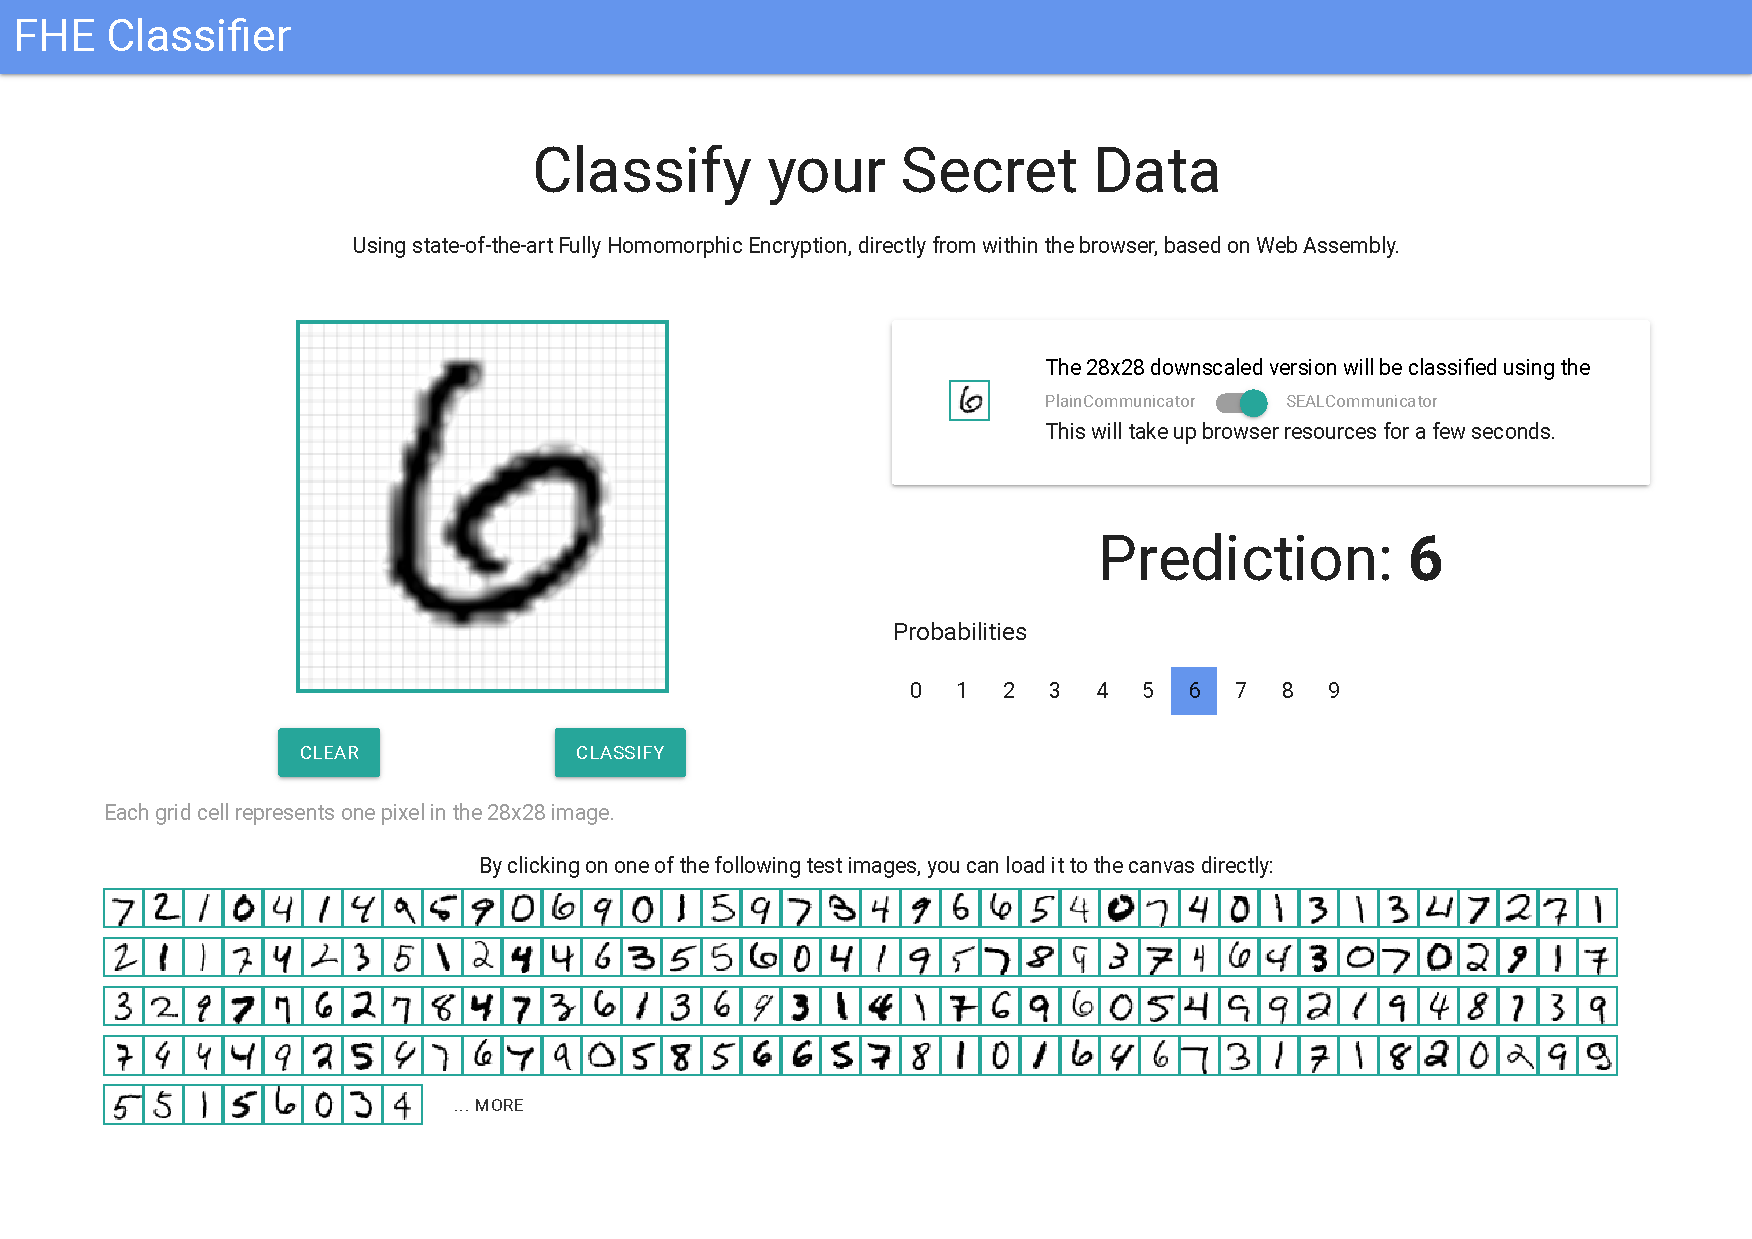
\includegraphics[width=0.75\linewidth]{../thesis/figures/frontend.pdf}
        \vspace{-0.3cm}
        \caption{\url{https://secure-classification.peter.waldert.at/}.}
      \end{figure}
    \end{column}
    \begin{column}{0.24\linewidth}
      Scan the QR-Code:
      \qrcode[nolink,height=3.1cm]{https://secure-classification.peter.waldert.at/}
    \end{column}
  \end{columns}
\end{frame}

\newcommand{\matmulscale}{0.75}
\newcommand{\matmulhoffset}{-3cm}
\begin{frame}{Matrix Multiplication: The Naïve Method}
  \begin{figure}[H]
    \centering
    \hspace{\matmulhoffset}
    \scalebox{\matmulscale}{\inputtikz{figures/generated/matmul-naive}}
    % \caption[Naïve matrix multiplication method]{The naïve method to multiply a matrix $M \in \R^{s \times t}$ with a vector $\vec{x} \in \R^t$ (adapted from \cite{2018-gazelle}).}
    \label{fig:naive-method}
  \end{figure}

  $$\{M \vec{x}\}_i = \sum_{j=1}^{t} M_{ij} x_j \,.$$
\end{frame}

\begin{frame}{Matrix Multiplication: The Diagonal Method}
  \begin{figure}[H]
    \centering
    \hspace{\matmulhoffset}
    \scalebox{\matmulscale}{\inputtikz{figures/generated/matmul-diagonal}}
    % \caption[Diagonal matrix multiplication method]{The diagonal method to multiply a square matrix with a vector (adapted from \cite{2018-gazelle}).}
    \label{fig:diagonal-method}
  \end{figure}

  $$M \vec{x} = \sum_{j=0}^{t-1} \diag_j(M) \cdot \rot_j(\vec{x}) \,.$$
\end{frame}

\begin{frame}{Matrix Multiplication: The Hybrid Method}
  \begin{figure}[H]
    \centering
    \hspace{\matmulhoffset}
    \scalebox{\matmulscale}{\inputtikz{figures/generated/matmul-hybrid}}
    % \caption[Hybrid matrix multiplication method]{The hybrid method to multiply an arbitrarily sized matrix with a vector (adapted from \cite{2018-gazelle}).}
    \label{fig:hybrid-method}
  \end{figure}

  $$M \vec{x} = (y_i)_{i \in \Z/s\Z} \;\text{with}\; \vec{y} = \sum_{k=1}^{t / s} \rot_{ks}\bigg(\sum_{j=1}^s \diag_j(M) \cdot \rot_j(\vec{x})\bigg) \,.$$
\end{frame}

\begin{frame}{Polynomial Evaluation}
  \begin{itemize}
    \item In between the dense layers, we need to evaluate the $\cryptop{relu}(x) := max(x, 0)$ function. \\
          $\Rightarrow$ Approximate it by a series expansion...
          $$\cryptop{relu\_taylor}(x) = -0.006137 x^3 + 0.090189 x^2 + 0.59579 x + 0.54738 \,.$$
    \item The \cryptop{softmax} activation at the end can be done by the client.
  \end{itemize}

  \begin{figure}[H]
    \centering
    \scalebox{0.56}{\inputtikz{figures/generated/taylor-relu}}
    \label{fig:taylor-relu}
  \end{figure}
\end{frame}

\begin{frame}{Runtime Benchmarks \& Communication Overhead}
  \begin{table}[H]
    \centering
    \setlength{\belowcaptionskip}{0pt}
    \caption[Performance Benchmarks / Communication Overhead]{
      Performance benchmarks and communication overhead of the classification procedure on an Intel\textregistered \, i7-5600U CPU, including the encoding and decoding steps.
    }
    % \captionsetup{margin=10pt}
    % \caption*{
    %   $\bm{B_1}$ ... Coefficient Moduli start bits (also equal to the last) \\
    %   $\bm{B_2}$ ... Coefficient Moduli middle bits, also defines the scale as $2^{B_2}$ \\
    %   $\bm{N}$ ... Polynomial Modulus Degree, found in the exponent of $p(X) = X^N + 1$ \\
    %   $\bm{T}$ ... Runtime of encryption + classification + decryption \\
    %   $\bm{M}$ ... Message Size (Relin Keys + Galois Keys + Request Ciphertext + Response Ciphertext) \\
    %   $\bm{\Delta}$ ... Mean Max-Relative Error compared to the exact result, i.e. $\bm{\Delta} := \frac{\langle |\bm{y}_{prediction} - \bm{y}_{exact}| \rangle}{\max |\bm{y}_{exact}|}$
    % }
    \SetTblrInner{rowsep=1pt}
    \scalebox{0.8}{
      \begin{tblr}{
        colspec={ccrrrr|rrr},
        row{2,3,4} = {bg=azure9},
        row{5,6,7} = {bg=violet9},
        row{8,9,10} = {bg=blue9},
        row{11,12,13} = {bg=azure9},
          }
        \hline
        \bf Mode & \bf SecLevel & $\bm{B_1}$ & $\bm{B_2}$ & $\bm{N}$ & \bf MatMul & $\bm{T}$ / \si{\second} & $\bm{M}$ / \si{\mebi\byte} & $\bm{\Delta}$ / 1 \\
        \hline
        & & & & & Diagonal & 8.39 & 132.72 & 0.0364 \\
        Release & tc128 & 34 & 25 & 8192 & Hybrid & 1.35 & 132.72 & 0.0362 \\
        & & & & & BSGS & 1.66 & 132.72 & 0.1433 \\
        \hline
        & & & & & Diagonal & 17.24 & 286.51 & 0.0363 \\
        & tc128 & 60 & 40 & 16384 & Hybrid & 3.05 & 286.51 & 0.0364 \\
        & & & & & BSGS & 3.66 & 286.51 & 0.1399 \\
        \hline
        & & & & & Diagonal & 35.24 & 615.16 & 0.0363 \\
        & tc256 & 60 & 40 & 32768& Hybrid & 5.99 & 615.16 & 0.0364 \\
        & & & & & BSGS & 7.34 & 615.16 & 0.1399 \\
      \end{tblr}
    }
    \label{tab:performance-benchmarks}
  \end{table}
  In Plain: 784 byte requests, taking \SI{50}{\micro\second}; Encrypted: \SI{132}{\mebi\byte} requests, taking \SI{1.4}{\second}.
\end{frame}

  \section{Step 5: Results and Accuracy}
\begin{frame}{Chaos everywhere: The Confusion Matrix}
  \centering
  \scalebox{0.64}{\inputtikz{figures/generated/confusion-matrix}}

  \vspace{-0.3cm}
  Plain Accuracy: \SI{97.6}{\percent}, Encrypted Accuracy: \SI{97.3}{\percent}.
\end{frame}

\begin{frame}{Ciphertext Visualisations}
  \begin{figure}[H]
    \centering
    \scalebox{0.9}{\inputtikz{figures/ciphertext-visualisation}}
    % \caption[Visualisation of the plain input images compared to their ciphertext]{Ciphertext Visualisation: The first row corresponds to the images in plain, the second row depicts an encrypted version, namely the reconstructed polynomial coefficients $\{a_k\}$ of the ciphertext polynomial.}
    \label{fig:ciphertext-visualisation}
  \end{figure}
\end{frame}

  \chapter{Conclusion}
\label{chap:conclusion}
\section{Summary}

\inputtikz{figures/venn-diagram}

\section{Outlook}
% describe existing solutions, approaches, current research, etc.
% -> list the papers in library/ folder?
% (include Fabians master thesis about splitting Relin, Galois keys using SPDZ
% to support multiple data providers (clients) and one server, using normal HE algorithms)

\section{Related Works}
Gazelle (inferred ML) as described by \cite{2018-gazelle}.

Random Forests (RF) on HE as described by \cite{2020-cryptotree}.


  \section*{}
  \begin{frame}[c]
    \centering
    \Large Questions?
  \end{frame}

  \begin{frame}[allowframebreaks]{Glossary}
    \printnoidxglossary[type=acronym]
  \end{frame}

  \begin{frame}[allowframebreaks]{Bibliography}
    \printbibliography
  \end{frame}

  \appendix
\titleformat{\chapter}[block]{\normalfont\LARGE\bfseries}{Appendix \thechapter \;\textendash\;}{0ex}{\vspace{-4cm}}[\vspace{4.5cm}]
\titlespacing{\chapter}{0cm}{0cm}{0cm}

\chapter{Supplemental Proofs}
\label{chap:appendix}

\section{Power-of-2 Cyclotomic Polynomials}
\label{proof:power-of-2-cyclo-poly}
\begin{proof}[Proof of \cref{thm:power-of-2-cyclo-poly}]
  With $k \in \N$ a positive integer, we want to show that
  $$\Phi_{2^k} (x) = x^{2^{k-1}} + 1\,.$$

  A polynomial $p \in \Z[X]$ with $$p(x) = x^n - a$$ of degree $n$ has $n$ roots
  $$\{x_j\} = \{a^\frac{1}{n} e^{2\pi i \frac{j}{n}} \,|\, j \in \N, j \leq n\}$$
  related by a factor $a^\frac{1}{n}$ to the \hyperref[lemma:nth-roots-of-unity]{$n$\textsuperscript{th} roots of unity} given by powers of $\xi = e^{2\pi i \frac{1}{n}}$.

  It is clear from the fundamental theorem of algebra that the polynomial $p$ with roots $\{x_j\}$ can be factorised as
  $$p(x) = \prod_{j=1}^{n} (x - x_j) = \prod_{j=1}^{n} (x - a^\frac{1}{n} e^{2\pi i \frac{j}{n}})\,.$$

  Fixing $a = -1$, we obtain $p(x) = x^n + 1$ with roots given by
  $$x_j = (-1)^\frac{1}{n} e^{2\pi i \frac{j}{n}}
    = (e^{i\pi})^\frac{1}{n} e^{2\pi i \frac{j}{n}}
    = e^{\frac{i\pi (2j + 1)}{n}}$$
  and according factorisation
  $$p(x) = \prod_{j=1}^{n} (x - e^{\frac{i\pi}{n} (2j + 1)})\,.$$

  Further letting $n = 2^{k-1}$ and observing that
  $$\gcd(2^k, l) = \begin{cases}
      1 & \text{if } l \text{ odd}  \\
      2 & \text{if } l \text{ even}
    \end{cases} \quad l, k \in \N$$
  since a number $2^k$ that can only be decomposed into multiples of $2$
  never shares a factor with an odd number, in accordance with \cref{lemma:nth-roots-of-unity}
  we can conclude that the set of all odd roots of unity is exactly the set of all primitive roots (satisfying $\gcd(2^k, l) = 1$).

  Following from above,
  \begin{align*}
    p(x) = \prod_{j=1}^{2^{k-1}} (x - e^{\frac{i\pi}{n} (2j + 1)})
    = \prod_{\stackrel{l=1}{l \text{ odd}}}^{2^k} (x - e^{\frac{i\pi}{n} l})
    = \prod_{\stackrel{l=1}{\xi^l \text{ primitive}}}^{2^k} (x - \xi^l)
    = \Phi_{2^k}(x)
  \end{align*}
  we arrive exactly at the definition of a cyclotomic polynomial (\cref{def:cyclotomic-poly}). \\
  \parencite{power-of-2-cyclo-poly}
\end{proof}

\section{Babystep-Giantstep Multiplication}
\label{proof:bsgs-matmul}
\begin{proof}[Proof of \cref{thm:bsgs}]
  Starting from the adapted \gls{bsgs} matrix-multiplication result $P = (P_1, P_2, ..., P_t)^T \in \R^t$, we want to show that we indeed end up with an authentic matrix-vector product.
  \begin{align*}
    P_i := \bigg\{\sum_{k=0}^{t_2-1} \rot_{(kt_1)} \big(
    \sum_{j=0}^{t_1-1} \diag'_{(kt_1+j)}(M) \cdot \rot_j(\vec{x})
    \big)\bigg\}_i = \sum_{k=0}^{t_2-1} \sum_{j=0}^{t_1-1} m'_{kt_1+j,(i+kt_1)} x_{(i+kt_1)+j}
  \end{align*}
  with
  \begin{align*}
    m'_{p,i} = \big\{ \diag'_p(M)\big \}_i = \big\{ \rot_{-\lfloor p/t_1 \rfloor \cdot t_1}(\diag_p(M)) \big\}_i
    = M_{i-\lfloor\frac{p}{t_1}\rfloor t_1, i-\lfloor\frac{p}{t_1}\rfloor t_1 + p}
  \end{align*}
  and therefore
  \begin{align*}
    m'_{kt_1+j,i}        & = M_{i-\lfloor\frac{kt_1+j}{t_1}\rfloor t_1, i-\lfloor\frac{kt_1+j}{t_1}\rfloor t_1 + kt_1+j} \\
                         & = M_{i-kt_1-\lfloor\frac{j}{t_1}\rfloor t_1, i-kt_1-\lfloor\frac{j}{t_1}\rfloor t_1 + kt_1+j} \\
                         & = M_{i-kt_1-\lfloor\frac{j}{t_1}\rfloor t_1, i+j-\lfloor\frac{j}{t_1}\rfloor t_1}             \\
    m'_{kt_1+j,(i+kt_1)} & = M_{i+kt_1-kt_1-\lfloor\frac{j}{t_1}\rfloor t_1, i+kt_1+j-\lfloor\frac{j}{t_1}\rfloor t_1}   \\
                         & = M_{i-\lfloor\frac{j}{t_1}\rfloor t_1, i+kt_1+j-\lfloor\frac{j}{t_1}\rfloor t_1}
  \end{align*}
  leading to
  \begin{align*}
    P_i = \sum_{k=0}^{t_2-1} \sum_{j=0}^{t_1-1} m'_{kt_1+j,(i+kt_1)} x_{(i+kt_1)+j}
    = \sum_{k=0}^{t_2-1} \sum_{j=0}^{t_1-1} M_{i-\lfloor\frac{j}{t_1}\rfloor t_1, i+kt_1+j-\lfloor\frac{j}{t_1}\rfloor t_1} x_{(i+kt_1)+j} \,.
  \end{align*}
  Noticing that the downward rounded fraction $\lfloor\frac{j}{t_1}\rfloor$ vanishes
  in a sum with $j$ running from $0$ to $t_1-1$, we can simplify to
  \begin{align*}
    P_i = \sum_{k=0}^{t_2-1} \sum_{j=0}^{t_1-1} M_{i,i+kt_1+j} x_{i+kt_1+j}
  \end{align*}
  which contains two sums running to $t_1$ and $t_2$ respectively, containing an expression of the form $k \cdot t_1 + j$, which allows us to condense the nested sums into one single summation expression, as $$\sum_{k=0}^{t_2-1} \sum_{j=0}^{t_1-1} f(kt_1+j) = \sum_{l=0}^{t-1} f(l)$$ indeed catches every single value $l \in \{0, 1, 2, ..., t=t_1 \cdot t_2\}$ with $l = kt_1+j$. \\
  In summary, we obtain
  \begin{align*}
    P_i & = \sum_{k=0}^{t_2-1} \sum_{j=0}^{t_1-1} M_{i,i+kt_1+j} x_{i+kt_1+j} \\
        & = \sum_{l=0}^{t-1} M_{i,i+l} x_{i+l}
    = \sum_{\nu=0}^{t-1} M_{i,\nu} x_{\nu}                                    \\
        & = \big\{M \vec{x}\big\}_i
  \end{align*}
  which indeed equals the conventional definition of a matrix-vector product.
\end{proof}

\end{document}
